\documentclass[class=article, crop=false]{standalone}
\usepackage[fleqn]{amsmath}
\usepackage{amssymb}
\usepackage{graphicx}
\graphicspath{ {../images/} }
\begin{document}

\section*{1D}
1D means that we are moving on a curve of fixed shape. We have 1 degree of freedom, therefore we only need 1 $\mathbb{R}$ parameter to fully describe the position of an object. We want to model the motion of the object (defined as position over time) so we need a function mapping time to a position. Both of these are modelled with real parameters so we have a function: \\
$x: \mathbb{R} \to \mathbb{R} \hspace*{1cm} t \mapsto x(t)$ \\\\

Displacement is change in position. From this we can draw 3 main graphs to graphically show motion, each with time as the x-axis. \\
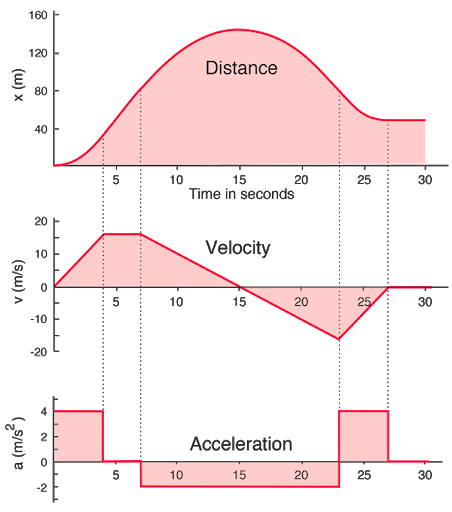
\includegraphics[scale=0.5]{Graphs1}

We can find the function representing the velocity and acceleration by taking the derivative and second derivative of the displacement/position time function respectively. \\
$v = \frac{dx}{dt} \hspace*{1cm} a = \frac{dv}{dt} = \frac{d^2x}{dt^2}$ \\
You can also go the other way and integrate them to get back to the displacement time function. \\
$v(t) - v(0)= \int_{t=0}^t a(t) dt \hspace*{1cm} x(t) - x(0) = \int_{t=0}^t v(t) dt$ \\\\

Average velocity is written $<v>$ or $\bar{v}$ and can be found by $\bar{v} = \frac{\Delta s(t)}{\Delta t}$. Similarly $\bar{a} = \frac{\Delta v(t)}{\Delta t}$ \\

\section*{SUVAT}
SUVAT is a set of equations modelling uniformly accelerating motion. The assumption is that $a(t) = a(0)$\\
The equations are:
\begin{align}
v & = u + at \\
s & = \frac{1}{2}(u + v)t \\
v^2 & = u^2 + 2as \\
s & = ut + \frac{1}{2}at^2 
\end{align}
Where $s$ represents displacement, $u$ is initial velocity, $v$ is final velocity, $a$ is acceleration and $t$ is time. \\
This produces graphs like this: \\
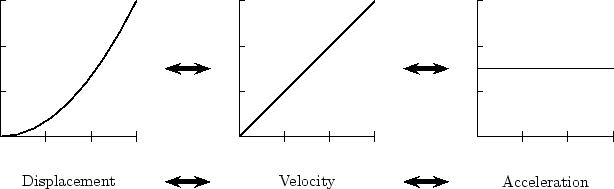
\includegraphics[scale=0.5]{Graphs2} \\
The SUVAT equations can be easily derived by integrating constant acceleration, although note that the integral only finds the change in a value rather than the absolute value. \\
In mechanics we treat an indefinite integral as the anti-derivative and just use definite integrals most of the time. 
\subsection*{Dimensions}
\begin{align*}
[s] & = \text{length } (m) \\
[t] & = \text{time } (s) \\
[v] & = [u] = \frac{[s]}{[t]} = [m.s^{-1}] \\
[a] & = \frac{[v]}{[t]} = \frac{[m.s^{-1]}}{[s]} = [m.s^{-2}] \\ 
\end{align*}
\section*{Forces and Newtons Laws}
In physics, forces model physical interaction between objects. E.g. Gravitational interaction, Electrostatic interaction, Strong nuclear force. \\
\subsection*{Modelling Forces Mathematically}
Forces have a magnitude and direction so the most basic model we can use is vectors. In more complex scenarios, for example with an extended (not a point particle) object or non rigid body they need to also have a line of action and may change the shape of the object so should be modelled with a vector field ($f:\mathbb{R}^3 \to \mathbb{R}^3$). \\
\paragraph*{Point Particle Model}
We can model objects as having all their mass concentrated at the center of mass to make them easier to study.
\subsection*{Force Diagrams}
We can represent forces using force diagrams showing the line of action and arrows to represent forces. Free body force diagrams are where we only consider the object in isolation and all the forces acting on it. \\
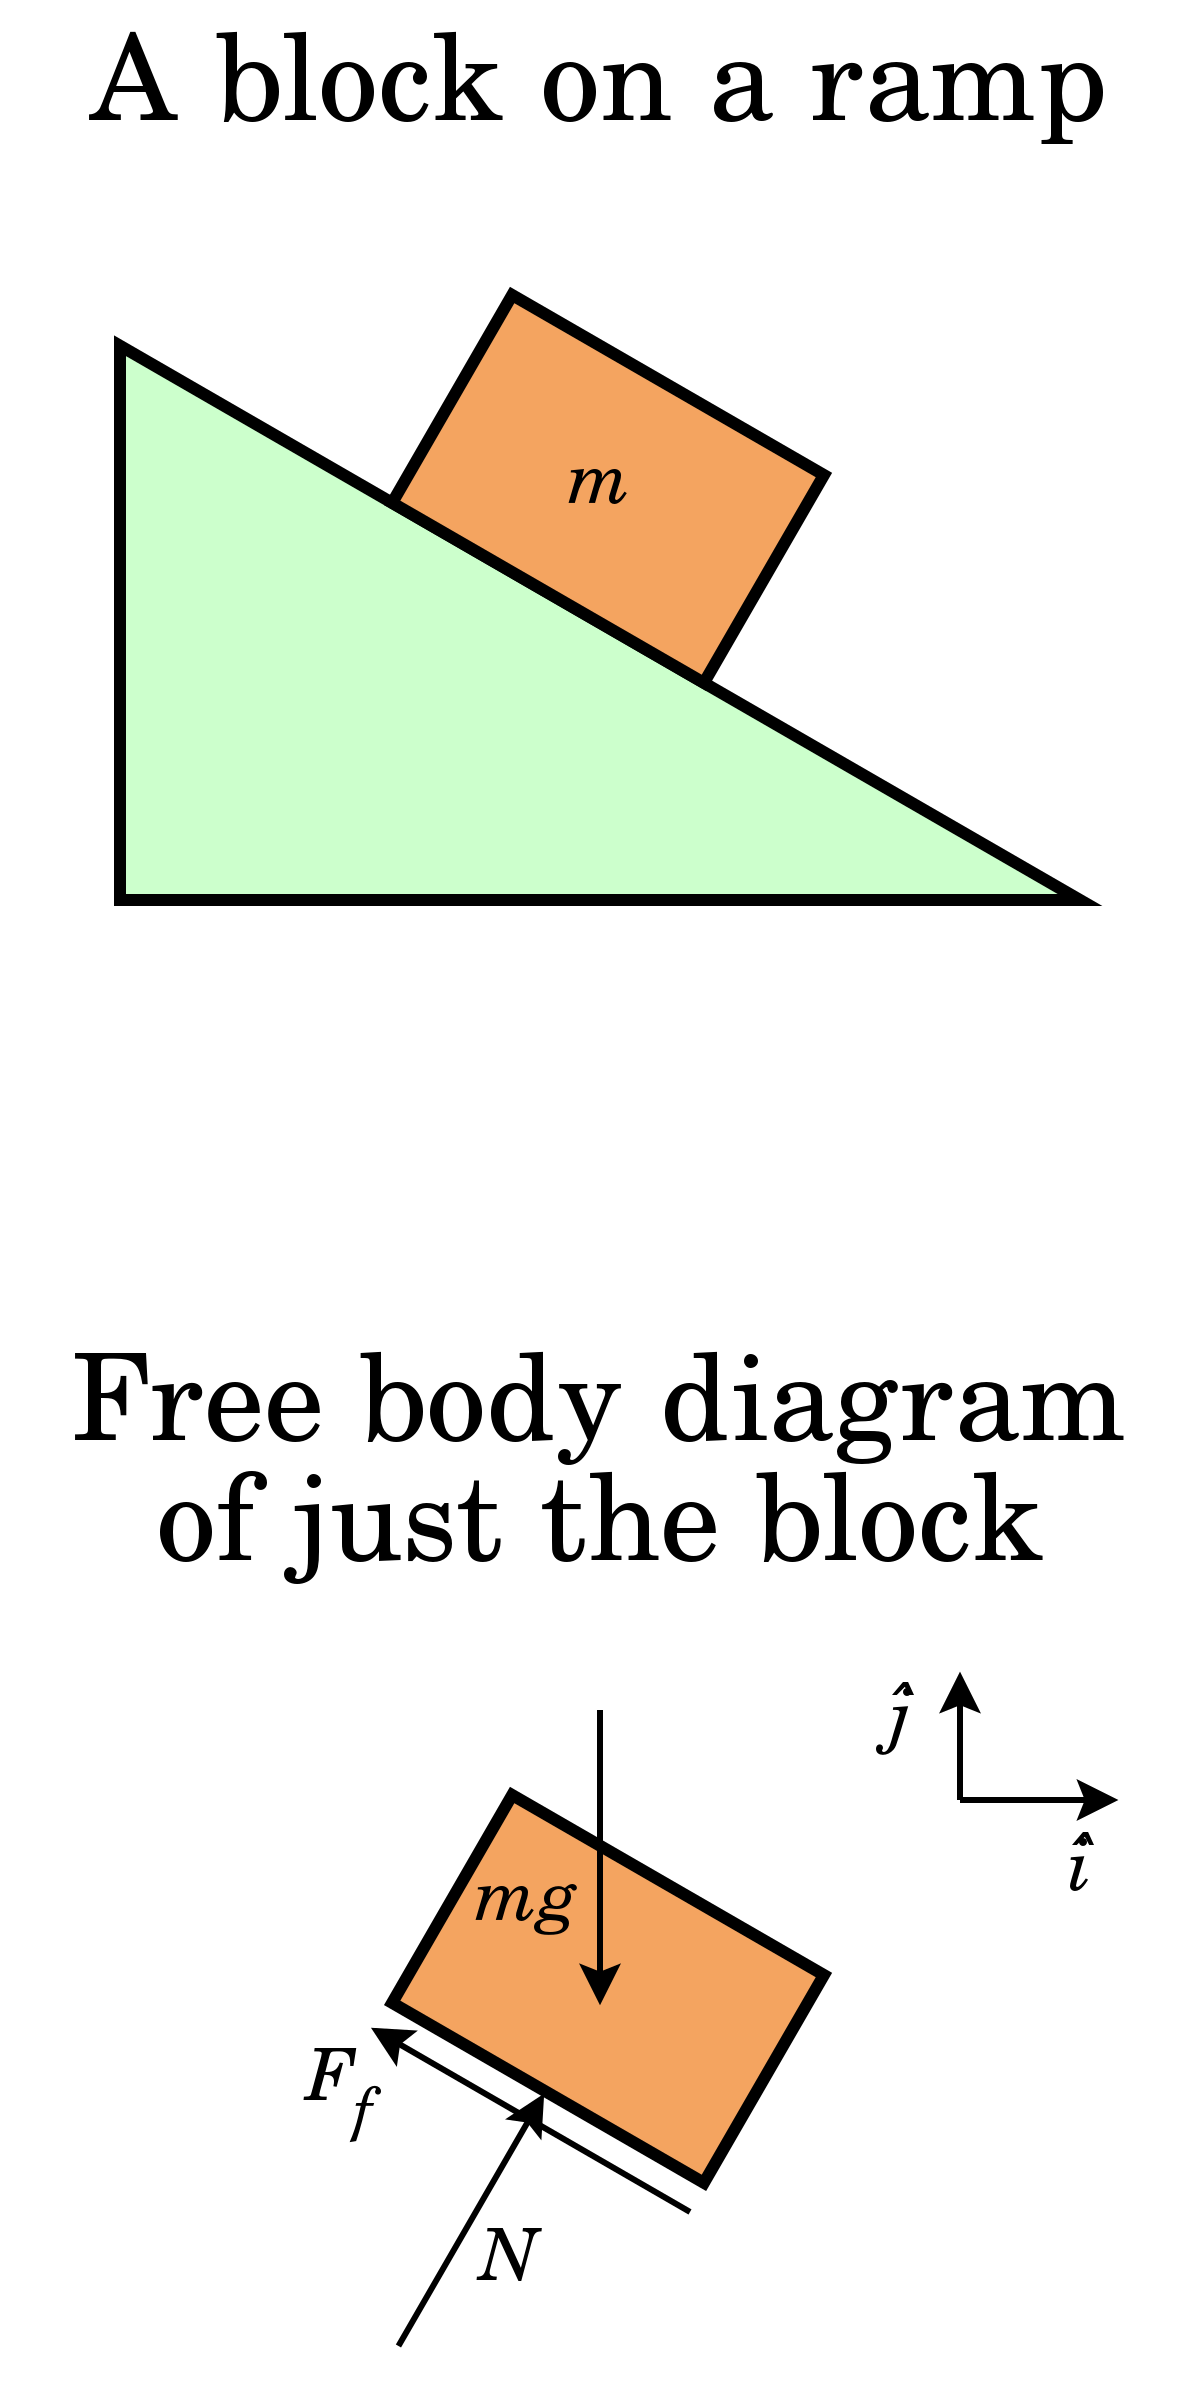
\includegraphics[scale=0.1]{ForceDiagram}\\
\subsection*{Newtons Laws}
\paragraph*{Newtons First Law}
Every particle continues in a state of rest or uniform motion in a straight line unless acted on by a resultant external force. \\\\
This also implies that a change in the velocity vector means that there is a force. 

\paragraph*{Newtons Second Law}
Change in motion is proportional to force. \\
\begin{align*}
& \dot{v} \propto F \Rightarrow a \propto F \\
& \Rightarrow ka = F \hspace*{1cm} k \propto \frac{1}{m} \\
& \Rightarrow F = ma \\
\end{align*}
This results in the definition of a newton: A mass of 1Kg accelerated by $1m.s^{-1}$

\paragraph*{Newtons Third Law}
When one object exerts a force on a other there is always a reaction of the same kind which is equal in magnitude and opposite in direction to the acting force. $\sum F \equiv 0$

\section*{Higher Dimensional}
In 2 or 3 dimensions, motion and forces must be modelled with vectors. We can use similar techniques for solving problems as before. This means that our displacement function must now map time to a point in 3 dimensional space so we get $x: \mathbb{R} \to \mathbb{R}^3$. \\

To find the derivative of a vector, it is just done component wise. 
\begin{align*}
x(t) & = \begin{bmatrix}
	x_1(t) \\
	x_2(t) \\
	x_3(t) \\
\end{bmatrix} \\
\Rightarrow \dot{x}(t) & = \begin{bmatrix}
	\dot{x}_1(t) \\
	\dot{x}_2(t) \\
	\dot{x}_3(t) \\
\end{bmatrix} \\
\end{align*}
\paragraph*{What does it means to integrate in higher dimensions?} To differentiate means to find the tangent. If we have a function mapping time to a velocity vector, to integrate it means to add up the instantaneous velocity and infinitesimal time steps. This means we are following where the velocity is going and therefore will end up with the displacement. We can also see that as integration is commutative with addition, that we will just need to do it component wise, like with differentiation. \\\\

The same techniques can be used to solve higher dimensional problems by just breaking down the motion in to individual components. 

\end{document}